\subsection{Testes}
\label{subsec:verificacao}

\subsubsection{Testes Unitários do Backend}

Status Atual: 458 testes em 57 suites, cobrindo os use cases críticos de todos os módulos, guards de autorização e fluxos de negócio complexos.

Padrão de Testes Adotado:
\begin{itemize}
\item AAA (Arrange-Act-Assert): Estrutura consistente em todas as suites.
\item makeMocks(): Cria todos os mocks via \texttt{jest.fn()} com tipagem \texttt{jest.Mocked<T>}.
\item setupHappyPath(): Configura mocks para o cenário de sucesso padrão.
\item Injeção manual: Dependências injetadas diretamente, sem mocks de framework NestJS.
\item Factories: Funções \texttt{make*()} por módulo com suporte a overrides parciais.
\end{itemize}

A Tabela~\ref{tab:testes} resume a quantidade de suites e testes por módulo; o detalhamento por use case está versionado no repositório (\texttt{test/modules/}).

\begin{table}[H]
\centering
\caption{Cobertura de testes unitários agregada por módulo}
\label{tab:testes}
\begin{tabular}{lrr}
\toprule
\textbf{Módulo} & \textbf{Suites} & \textbf{Testes} \\
\midrule
Trip & 18 & 183 \\
Bookings & 9 & 88 \\
Auth & 7 & 36 \\
Driver & 4 & 33 \\
Shared (Guards) & 3 & 26 \\
Payment & 3 & 20 \\
Subscriptions & 3 & 18 \\
Scheduling & 2 & 15 \\
Membership & 1 & 10 \\
Organization & 2 & 10 \\
Vehicle & 2 & 7 \\
User & 2 & 6 \\
Plans & 1 & 6 \\
\midrule
\textbf{Total} & \textbf{57} & \textbf{458} \\
\bottomrule
\end{tabular}
\end{table}


Os testes apoiam-se em \textit{factories} por módulo (funções \texttt{make*()} com suporte a \textit{overrides} parciais) que constroem entidades de domínio e DTOs de entrada, por exemplo \texttt{makeUser}, \texttt{makeOrganization}, \texttt{makeDriver}, \texttt{makeTripTemplate}, \texttt{makeTripInstance}, \texttt{makeBooking}, \texttt{makeSubscription}, eliminando duplicação de \textit{setup} entre as suites.

Complementarmente à contagem de testes, a Figura~\ref{fig:cobertura} apresenta o relatório de cobertura gerado pelo Jest, com os percentuais de \textit{statements}, \textit{branches}, \textit{functions} e \textit{lines} por módulo. A cobertura concentra-se nos módulos de maior criticidade de negócio, com destaque para \textit{bookings}, \textit{trip} e \textit{auth}, refletindo a priorização deliberada dos casos de uso centrais do sistema; a ampliação da cobertura dos módulos secundários consta entre as limitações e recomendações (Seção~\ref{sec:consideracoes}).

\begin{figure}[H]
\centering
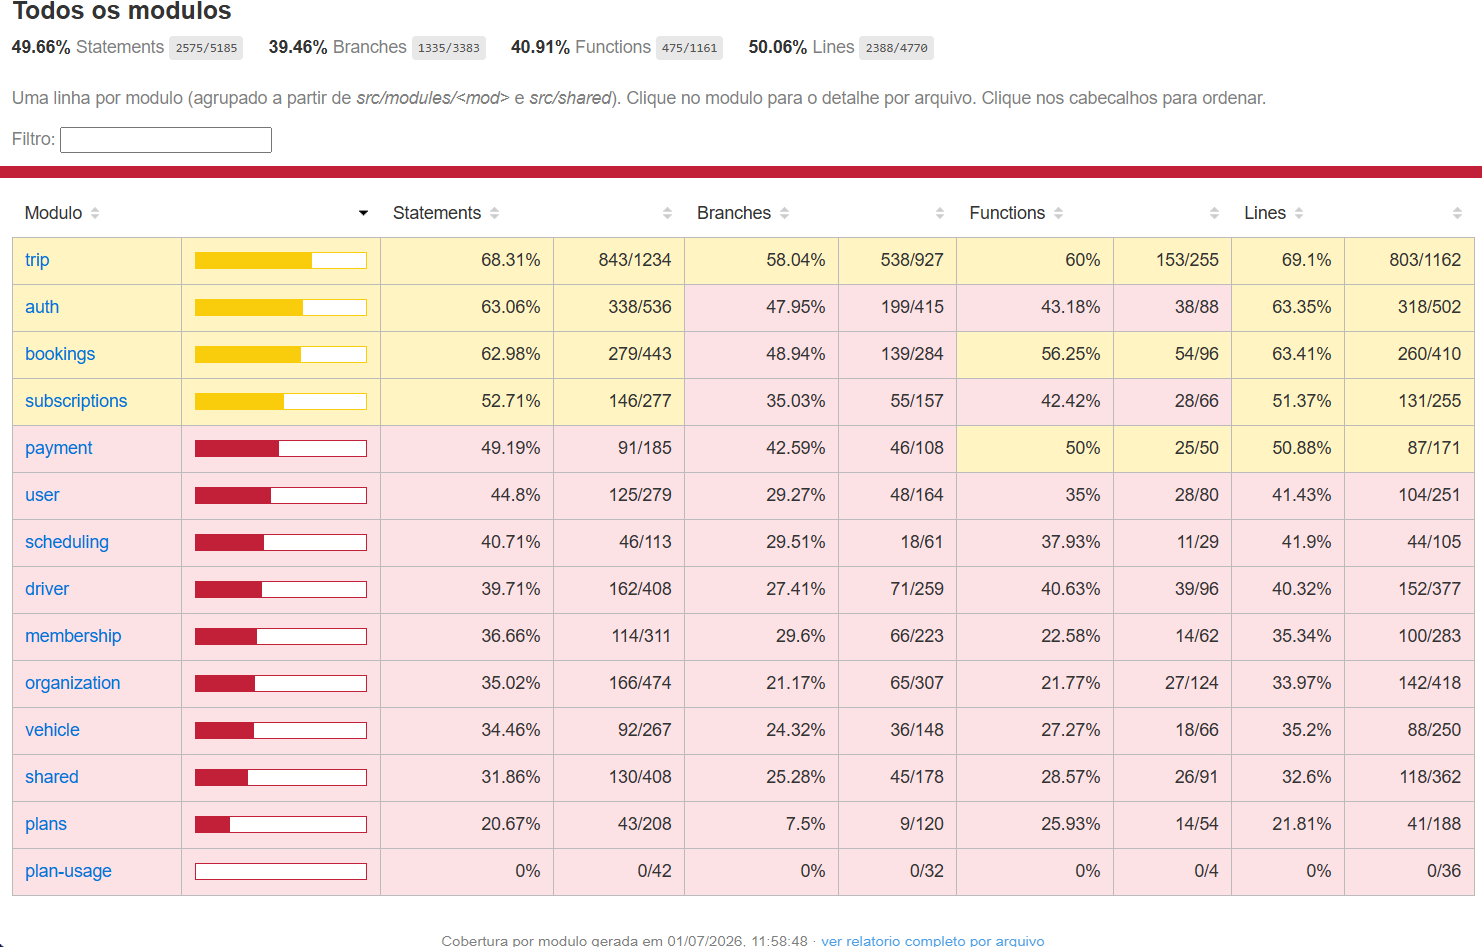
\includegraphics[width=\textwidth]{imagens/jest-coverage-completo.png}
\caption{Relatório de cobertura de testes do \textit{backend} (Jest), agregado por módulo.}
\label{fig:cobertura}
\end{figure}

\subsubsection{Verificação do Frontend}

Em coerência com o estágio do produto e o tamanho reduzido da equipe, a estratégia de verificação do frontend é, no momento, predominantemente manual, estruturada em um roteiro de dezenas de cenários que cobrem os caminhos principais, os fluxos que cruzam contextos de acesso e os casos de borda. A integração contínua executa a verificação de estilo, a análise estática e a construção, deixando a verificação funcional a cargo do roteiro manual. A adoção de testes automatizados (provavelmente Vitest com \textit{Testing Library} para \textit{hooks} e serviços, e uma ferramenta de ponta a ponta para os fluxos) está condicionada à aproximação da operação comercial, tendo o fluxo de reserva como primeiro candidato à cobertura. A Tabela~\ref{tab:testes_manuais} ilustra o formato dos casos de teste manuais.

\begin{table}[H]
\centering
\caption{Exemplos de casos de teste manuais do frontend}
\label{tab:testes_manuais}
\begin{tabular}{lll}
\toprule
\textbf{Caso} & \textbf{Resultado esperado} & \textbf{Status} \\
\midrule
Login com credenciais válidas & Sessão criada e redirecionamento por papel & OK \\
Login com credenciais inválidas & Mensagem de erro, sem sessão & OK \\
Expiração do \textit{token} durante navegação & Renovação transparente, ação concluída & OK \\
Mesmo ponto de embarque e desembarque & Bloqueio com mensagem de validação & OK \\
Cancelamento fora da janela permitida & Bloqueio com mensagem do \textit{errorCode} & OK \\
Rota administrativa sem papel de admin & Redirecionamento para a raiz & OK \\
\bottomrule
\end{tabular}
\end{table}

% ------------------------------
